\chapter{Analysis strategy\label{sec:strategy}}

\section{Search signature\label{sec:signature}}
The signal studied in this analysis is the production of an SM-like Higgs boson $H$ followed by its decay to a pair of lighter pseudoscalar Higgs bosons $a$, each of which decays to a pair of taus. Due to the large mass difference between $H$ and $a$, the $a$'s are produced with a large boost. Four production channels (Figure~\ref{fig:signatures}) for the $H$ are considered: $W$ and $Z$ associated production (WH and ZH), where a high-$p_T$ isolated muon from the vector boson decay provides a convenient trigger, gluon fusion (ggH), and vector boson fusion (VBF). The analysis was originally optimized for the WH mode but is sensitive to the ggH+VBF mode due to its large cross section. Since no forward jet tagging is done, the analysis is only sensitive to the sum of ggH and VBF, not each mode individually.  One of the $\tau\tau$ pairs is identified via the $\tau_{\mu}\tau_{\text{had}}$ decay topology, while no selection is made on the other $\tau\tau$ pair. The most significant backgrounds to the signal are expected to be SM $W$ and Drell-Yan production, where the $W$ and $Z$ decay to muons; $t\bar{t}$ with one or two muons in the final state; and heavy flavor QCD. In all of these backgrounds, the boosted $\tau_{\mu}\tau_{\text{had}}$ pair is faked by a jet.

\begin{figure}[hbtp]
  \begin{center}
    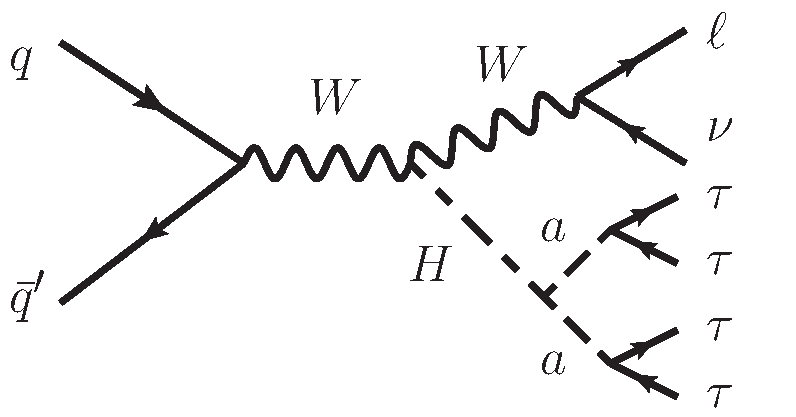
\includegraphics[width=\cmsFigWidth]{figures/FeynWH_ellnu4tau}
    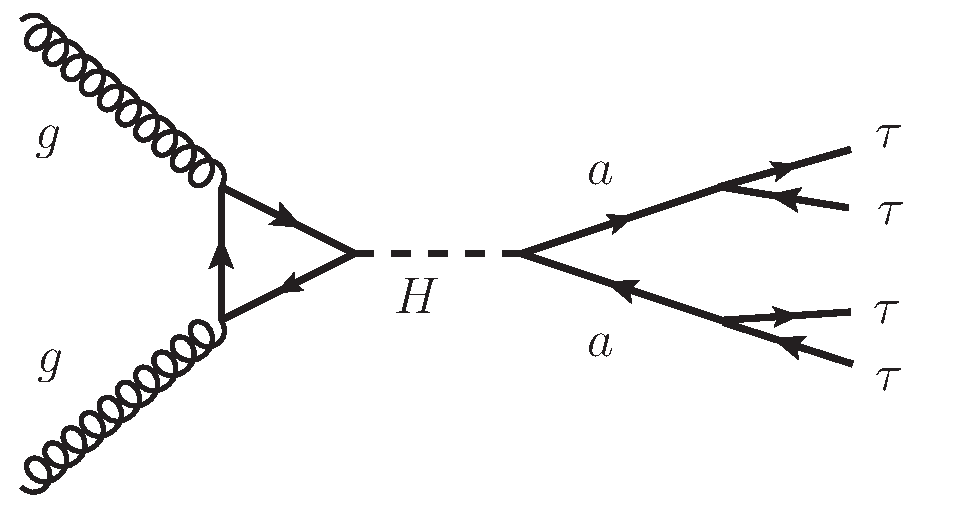
\includegraphics[width=\cmsFigWidth]{figures/FeynggH_aa_4tau}
    \caption{Feynman diagrams of signal processes. (\cmsLeft) $W$ associated production channel. (\cmsRight) Gluon fusion production channel.}
    \label{fig:signatures}
  \end{center}
\end{figure}

\section{Motivations\label{sec:motivations}}

\subsection{Light pseudoscalars\label{sec:lighta}}
% Explain how some models allow light (pseudo)scalars, under what conditions this can occur, and what the expected cross-sections are --> ask Jack.
Following the discovery by the CMS and ATLAS experiments at the LHC~\cite{Aad:2012tfa,Chatrchyan:2012ufa} of a Higgs-like particle $H$, additional measurements of its properties using the full data sets at $\sqrt{s}$ = 7 and 8 TeV reveal that the observed state with a mass near 125.5 GeV is quite consistent with the standard model (SM)~\cite{ATLASnew,CMS:new,Aad:2013wqa}. It is thus clear that models with an extended Higgs sector are significantly constrained by the data.  Consequently, it is interesting to explore the important possibility~\cite{Dermisek:2005ar,Dermisek:2006wr} that decays of the type $H$$\rightarrow$$aa$ (where $a$ is a lighter pseudoscalar) or $H$$\rightarrow$$hh$ (where $h$ is a lighter scalar) are present (for reviews, see~\cite{Chang:2008cw,Curtin:2013fra}). Such decays are certainly possible in the context of various extensions of the SM, including two Higgs doublet models (2HDM), the next-to-minimal supersymmetric standard model (NMSSM), and purely Higgs-sector models containing additional singlet Higgs fields, but notably are not possible in the (CP-conserving) minimal supersymmetric standard model (MSSM) because of the tightly constrained nature of its Higgs sector. 2HDM studies that consider, at least briefly, the possible decays of the observed SM-like Higgs to a pair of lighter Higgs bosons include~\cite{Celis:2013rcs,Grinstein:2013npa,Coleppa:2013dya,Chen:2013rba,Craig:2013hca,Wang:2013sha,Curtin:2013fra,Baglio:2014nea}. Studies in the NMSSM or NMSSM-like context include~\cite{King:2012tr,Cao:2013gba,Christensen:2013dra,Cerdeno:2013cz,Curtin:2013fra} and studies in the general case of adding a singlet field to the SM or the 2HDM can be found in~\cite{Chalons:2012qe,Ahriche:2013vqa,Curtin:2013fra}.

The branching ratio for the $H$ to decay to two lighter Higgs bosons is limited by the apparently SM-like nature of the $H$. An often-studied option is that of $H$ decays to invisible states. However, limits obtained under the assumption of invisibility do not apply to Higgs pair states, which should rather be thought of as simply unseen, $U$, decay modes. The most thorough study for this case is that of~\cite{Belanger:2013xza} which combines CMS and ATLAS data. There it is found at 95\% C.L. that: Br($H$$\rightarrow$$U$) $\le$ 0.21 for a Higgs with completely SM-like couplings; Br($H$$\rightarrow$$U$) $\le$ 0.31 for a SM Higgs but allowing for extra loop contributions to its $\gamma\gamma$ and gg couplings; and Br($H$$\rightarrow$$U$) $\le$ 0.39 if the couplings to up quarks, down quarks and vector bosons are allowed to vary within a general model with only doublets and singlets in the Higgs sector (and no extra loop contributions to the gg and $\gamma\gamma$ couplings). If the up, down and vector boson couplings are allowed to vary completely freely, then all LHC rates can be reproduced if all the couplings-squared are increased by a factor of 1/(1-Br($H$$\rightarrow$$U$)). The only limit in this latter case arises from direct limits on the observed Higgs total width.  At the moment, this is at the level of $\Gamma_{\text{tot}} \le 4\Gamma_{\text{tot}}^{\text{SM}}$~\cite{CMSHwidth}. If the couplings-squared are all increased by 1/(1-Br($H$$\rightarrow$$U$)), the rates for $gg$$\rightarrow$$H$$\rightarrow$$U$ and other production mechanisms are all increased by a factor of Br($H$$\rightarrow$$U$)/(1-Br($H$$\rightarrow$$U$)), making such modes even more accessible. However, even if one adopts the more conservative approach of only considering doublets+singlets models, there is still an excellent prospect for seeing Higgs pair modes if Br($H$$\rightarrow$$U$) $\la$ 0.39.  

Indeed, almost any branching ratio for $H$$\rightarrow$$aa$ or $H$$\rightarrow$$hh$ is possible and imposing Br($H$$\rightarrow$$U$) $\la$ 0.39 significantly constrains 2HDM+singlets theories.  This is because the required $H$$\rightarrow$$aa$ or $H$$\rightarrow$$hh$ couplings are inevitably present and are generically sizeable, and are sufficiently large that to avoid $\Gamma$($H$$\rightarrow$$aa$,$hh$) $\gg$ $\Gamma$($H$$\rightarrow$$b\bar{b}$) requires significant parameter tuning (assuming $m_a$, $m_h$ < $m_H$/2). For example, in the NMSSM (where the pseudoscalar mass eigenstate is defined by $a$ = $\cos\theta_A$ $a_{\text{MSSM}}$ + $\sin\theta_A$ $a_S$, with $a_{\text{MSSM}}$ being the MSSM-like pseudoscalar and $a_S$ the singlet pseudoscalar of the NMSSM). $\abs{\cos\theta_A}$ $\ll$ 1 is generically needed to keep the Haa coupling small by suppressing the doublet content of the $a$.  In the 2HDM, fine-tuned relations among the parameters of the model are required for acceptably small ($\la 0.2$) Br($H$$\rightarrow$$aa$) or Br($H$$\rightarrow$$hh$).

Direct constraints on the $a$ or $h$ play a role in assessing the possibilities. A previous CMS result~\cite{Chatrchyan:2012am} (based on~\cite{Dermisek:2009fd}) places limits on $\sigma$($pp$$\rightarrow$$aa$$\rightarrow$$\mu\mu$) on the order of 2\mdash6 pb in the mass range from 5\mdash14 GeV, excluding the upsilon resonance region.  These limits, despite being based on just 1.3 fb$^{-1}$ of 7 TeV data, can impact models. For example,~\cite{Chatrchyan:2012am} shows that they significantly constrain the $\cos\theta_A$ mixing angle factor defining the NMSSM.  The constraints on $\abs{\cos\theta_A}$ are especially strong at large $\tan\beta$, where $\tan\beta$ is defined as the ratio of the neutral Higgs vacuum expectation values in the MSSM. In the case of the single $a$ = $a_{\text{MSSM}}$ state of the CP-conserving 2HDM, points in the parameter space that are consistent with $m_H \sim$ 125.5 GeV fits at 95\% C.L. and other LHC and pre-LHC constraints violate this limit in the case of Type~II models (but not in the case of Type~I)~\cite{Dumont:2014wha}.  However, in general such constraints do not significantly restrict Br($H$$\rightarrow$$aa$) or Br($H$$\rightarrow$$hh$).  

The techniques appropriate for detecting a Higgs-pair decay mode depend crucially on the mass of the lighter Higgs boson. One important possibility, particularly prominent in the NMSSM, is that the lightest CP-odd state $a$ has mass below or not far above $2m_b$. Small $m_a$ arises naturally in the limit of a so-called $U(1)_R$ symmetry of the model. However, a small mass for the light Higgs states is generically possible in all the models listed earlier. In addition, even if the light Higgs boson has mass above $2m_b$ (but, of course, below $m_H$/2) the $\tau\tau$ mode will still have a branching ratio of order 0.045 and will have smaller backgrounds than a purely 4$b$ final state or the $b\bar{b}\tau\tau$ final state. Thus, a generic exploration of the sensitivity in the $4\tau$ final state is of considerable interest, especially as more and more integrated luminosity is accumulated in future running.

\subsection{Semileptonic di-tau decays\label{sec:semileptonic}}
This analysis explores the current level of sensitivity to the $4\tau$ final state, and techniques are developed for isolating this final state from backgrounds. In particular, at least one of the tau pairs produced in the decays of the light Higgs bosons is required to decay semileptonically as $\tau_{\mu}\tau_{\text{had}}$. Requiring at least one hadronic tau decay is intended to maximize statistics, due to the higher branching ratio for hadronic tau decays -- 64.76\% compared to 17.41\% and 17.83\% for decays to muons or electrons respectively~\cite{Agashe:2014kda}. However, the choice for the other tau not to decay hadronically was motivated by issues with the reconstruction of boosted tau pairs.

Because of the large mass difference between the $H$ and $a$, the final-state tau pairs are highly collimated, resulting in the overlap of their decay products. This spoils the isolation of the individual taus and renders their reconstruction difficult or impossible by standard means. In order to reconstruct boosted $\tau\tau$ pairs, a modified version of the standard hadron plus strips (HPS)~\cite{CMS:2011msa} tau reconstruction procedure has been developed for this analysis. This method, described fully in Section~\ref{sec:evtsel-tauID}, involves identifying and removing a leptonic tau decay candidate (muon or electron) from the PF jet used to seed the hadronic tau decay reconstruction. As this method has been successful in recovering hadronic tau ID efficiency, this analysis has thus focused on the reconstruction of semileptonic boosted tau decays -- in particular, only $\tau_{\mu}\tau_{\text{had}}$ decays, due to the relative ease and cleanness with which low-$p_T$ muons are reconstructed at CMS compared to electrons.

\section{Datasets\label{sec:datasets}}
%%%%%%%%%%%%%%%%%%%

\subsection{Data samples and trigger\label{sec:datasets-data}}
The datasets used in this analysis are the most recent \texttt{SingleMu} primary datasets collected by CMS in 2012 at $\sqrt{s}$ = 8 TeV.  The high level trigger (HLT) path \texttt{HLT\_IsoMu24\_eta2p1} requires the presence of at least one isolated muon with $p_T >$ 24 GeV found within the CMS muon coverage of $\abs{\eta} <$ 2.1.  More details about the HLT muon reconstruction and isolation requirement can be found in Ref.~\cite{HLTMenus}.  These datasets, listed in Table~\ref{tab:Data}, correspond to an integrated luminosity of 19.7 fb$^{-1}$. The JSON file used in the analysis for bad data masking can be found at \texttt{/afs/cern.ch/cms/CAF/CMSCOMM/COMM\_DQM/certification/Collisions12/8TeV/\\Reprocessing/Cert\_190456-208686\_8TeV\_22Jan2013ReReco\_Collisions12\_JSON.\\txt}.

\begin{table}
\begin{center}
\singlespacing
\begin{tabular}{ll}
	\hline
	Dataset name & Run range \\
	\hline
	\texttt{/SingleMu/Run2012A-22Jan2013-v1/AOD} & 190456-193621 \\
	\texttt{/SingleMu/Run2012B-22Jan2013-v1/AOD} & 193833-196531 \\
	\texttt{/SingleMu/Run2012C-22Jan2013-v1/AOD} & 198022-203742 \\
	\texttt{/SingleMu/Run2012D-22Jan2013-v1/AOD} & 203777-208686 \\
	\hline
\end{tabular}
\caption{Data samples.}
\label{tab:Data}
\end{center}
\end{table}

\subsection{Monte Carlo samples\label{sec:datasets-MC}}
The Monte Carlo (MC) samples used for the backgrounds outlined in the introduction are listed in Table~\ref{tab:MCBkg}.

\begin{sidewaystable}
\begin{center}
\caption{Monte Carlo background samples. Cross sections from \cite{PREP} and \cite{8TeVTwiki}.\label{tab:MCBkg}}
\singlespacing
\resizebox{\textwidth}{!}{\begin{tabular}{| l | l |}
        \hline
	Dataset name & \begin{tabular}[c]{@{}l@{}}Cross \\section (pb)\end{tabular} \\
	\hline
	\hline
	\texttt{/W1JetsToLNu$\_$TuneZ2Star$\_$8TeV-madgraph/Summer12$\_$DR53X-PU$\_$S10$\_$START53$\_$V7A-v1/AODSIM} & 6601.5 \\
	\texttt{/W2JetsToLNu$\_$TuneZ2Star$\_$8TeV-madgraph/Summer12$\_$DR53X-PU$\_$S10$\_$START53$\_$V7A-v1/AODSIM} & 2110.3 \\
	\texttt{/W3JetsToLNu$\_$TuneZ2Star$\_$8TeV-madgraph/Summer12$\_$DR53X-PU$\_$S10$\_$START53$\_$V7A-v1/AODSIM} & 633.6 \\
	\texttt{/W4JetsToLNu$\_$TuneZ2Star$\_$8TeV-madgraph/Summer12$\_$DR53X-PU$\_$S10$\_$START53$\_$V7A-v1/AODSIM} & 214 \\
	\texttt{/DYJetsToLL$\_$M-10To50$\_$TuneZ2Star$\_$8TeV-madgraph/Summer12$\_$DR53X-PU$\_$S10$\_$START53$\_$V7A-v1/AODSIM} & 14702 \\
	\texttt{/DYJetsToLL$\_$M-50$\_$TuneZ2Star$\_$8TeV-madgraph-tarball/Summer12$\_$DR53X-PU$\_$S10$\_$START53$\_$V7A-v1/AODSIM} & 3503.71 \\
	\texttt{/TTJets$\_$MassiveBinDECAY$\_$TuneZ2star$\_$8TeV-madgraph-tauola/Summer12$\_$DR53X-PU$\_$S10$\_$START53$\_$V7A-v2/AODSIM} & 245.8 \\
	\texttt{/T$\_$s-channel$\_$TuneZ2star$\_$8TeV-powheg-tauola/Summer12$\_$DR53X-PU$\_$S10$\_$START53$\_$V7A-v1/AODSIM} & 3.79 \\
	\texttt{/T$\_$t-channel$\_$TuneZ2star$\_$8TeV-powheg-tauola/Summer12$\_$DR53X-PU$\_$S10$\_$START53$\_$V7A-v1/AODSIM} & 56.4 \\
	\texttt{/Tbar$\_$s-channel$\_$TuneZ2star$\_$8TeV-powheg-tauola/Summer12$\_$DR53X-PU$\_$S10$\_$START53$\_$V7A-v1/AODSIM} & 1.76 \\
	\texttt{/Tbar$\_$t-channel$\_$TuneZ2star$\_$8TeV-powheg-tauola/Summer12$\_$DR53X-PU$\_$S10$\_$START53$\_$V7A-v1/AODSIM} & 30.7 \\
	\texttt{/WW$\_$TuneZ2star$\_$8TeV$\_$pythia6$\_$tauola/Summer12$\_$DR53X-PU$\_$S10$\_$START53$\_$V7A-v1/AODSIM} & 54.838 \\
	\texttt{/WZ$\_$TuneZ2star$\_$8TeV$\_$pythia6$\_$tauola/Summer12$\_$DR53X-PU$\_$S10$\_$START53$\_$V7A-v1/AODSIM} & 33.21 \\
	\texttt{/ZZ$\_$TuneZ2star$\_$8TeV$\_$pythia6$\_$tauola/Summer12$\_$DR53X-PU$\_$S10$\_$START53$\_$V7A-v1/AODSIM} & 17.654 \\
	\hline
\end{tabular}}
\end{center}
\end{sidewaystable}

The Monte Carlo signal samples for associated WH production and gluon fusion production were generated with PYTHIA~\cite{1126-6708-2006-05-026} and reconstructed with CMSSW version 5.3 using the \texttt{S10} pileup scenario. The $W$ in the associated $W$ production sample is constrained to decay only leptonically. Since PYTHIA does not model NMSSM processes, the production and decay of the NMSSM scalar and pseudoscalar Higgs particles were approximated using PYTHIA's two Higgs doublet model instead. A separate sample of signal events was generated using MADGRAPH~\cite{springerlink:10.1007/JHEP06(2011)128}, which does contain methods for modeling NMSSM processes directly, and the kinematics of the PYTHIA and MADGRAPH event samples were shown to be compatible and equivalent. The benchmark for this analysis takes the masses of the NMSSM $a$, $h_1$, $h_2$, and $h_3$ to be 9, 125, 500, and 500 GeV respectively; a mass scan is performed over $m_{a}$ from 5 to 15 GeV in increments of 2 GeV.  The assumed cross sections for each signal sample are given in Table~\ref{tab:MC-sig}.  These are the cross sections for SM 125 GeV Higgs production at 8 TeV~\cite{LHCHXSWG} multiplied by BR($H\rightarrow$$aa\rightarrow4\tau$) = 100\%, which is why the cross sections are constant with pseudoscalar mass.  The $W\rightarrow$ leptons branching ratio is included in the quoted cross sections for the WH signals.

\begin{table*}[htbh]
\begin{center}
\caption{Assumed signal MC cross sections.\label{tab:MC-sig}}
\singlespacing
\begin{tabular}{|c|c|c|}
\hline
\multicolumn{2}{|c|}{} & Cross section (pb) \\
\hline
\multirow{5}{*}{WH} & $m_{a}$ = 5 GeV & 0.2296\\
& $m_{a}$ = 7 GeV & 0.2296\\
& $m_{a}$ = 9 GeV & 0.2296\\
& $m_{a}$ = 11 GeV & 0.2296\\
& $m_{a}$ = 13 GeV & 0.2296\\
& $m_{a}$ = 15 GeV & 0.2296\\
\hline
\multirow{5}{*}{ggH} & $m_{a}$ = 5 GeV & 19.27\\
& $m_{a}$ = 7 GeV & 19.27\\
& $m_{a}$ = 9 GeV & 19.27\\
& $m_{a}$ = 11 GeV & 19.27\\
& $m_{a}$ = 13 GeV & 19.27\\
& $m_{a}$ = 15 GeV & 19.27\\
\hline
\multirow{5}{*}{ZH} & $m_{a}$ = 5 GeV & 0.4153\\
& $m_{a}$ = 7 GeV & 0.4153\\
& $m_{a}$ = 9 GeV & 0.4153\\
& $m_{a}$ = 11 GeV & 0.4153\\
& $m_{a}$ = 13 GeV & 0.4153\\
& $m_{a}$ = 15 GeV & 0.4153\\
\hline
\multirow{5}{*}{VBF} & $m_{a}$ = 5 GeV & 1.578\\
& $m_{a}$ = 7 GeV & 1.578\\
& $m_{a}$ = 9 GeV & 1.578\\
& $m_{a}$ = 11 GeV & 1.578\\
& $m_{a}$ = 13 GeV & 1.578\\
& $m_{a}$ = 15 GeV & 1.578\\
\hline
\end{tabular}
\end{center}
\end{table*}

\subsection{Higgs transverse momentum reweighting for ggH\label{sec:datasets-higgsptreweight}}

In gluon fusion Higgs production, the Higgs $p_T$ spectrum can be significantly affected by next-to-leading logarithmic (NLL) and next-to-next-to-leading logarithmic (NNLL) corrections, especially in the low-$p_T$ range~\cite{Bozzi:2003jy}. Thus, a set of weights binned in $p_T$, calculated with the Higgs $p_T$-reweighting HqT software \cite{HQTDocumentation}, was applied to the Higgs $p_T$ spectrum of signal MC events in the ggH production channel. The effect of this reweighting was observed to be quite small, as it produced a change of less than 2\% in signal-to-background ratio for each signal and a change of less than 2.5\% in the number of each type of signal event passing the final selection.

\subsection{ZH and VBF production channels\label{sec:datasets-zhvbf}}

A study was done to assess the contribution of ZH and VBF production channels to the expected signal significance. ZH and VBF signal samples were generated for pseudoscalar mass point $m_{a}$ = 9 GeV and the numbers of events passing the analysis selection sequence were normalized to 19.7 fb$^{-1}$ using the official SM production cross sections for ZH and VBF. Then, expected limits for the WH and ggH signal channels were calculated after the total expected yield of ZH and VBF events was distributed among the WH and ggH expected yields proportionally to their sizes, and these expected limits were compared to the nominal expected limits for WH and ggH without the added events. The combined presence of ZH and VBF signals changed the WH and ggH expected limits by at most 10\%, and the change was always well within the $1\sigma$ error band of the nominal expected limits. Yet, in the low-$M_{T}$ bin, the contribution of VBF was larger than that of WH, so ultimately it was concluded that the contributions of VBF and ZH should be considered too.

However, due to a shortage of time, ZH and VBF MC samples could not be generated for the other pseudoscalar mass points. Instead, the contribution of VBF for each pseudoscalar mass point was estimated by taking the number of surviving ggH events in the counting experiment bin after the full selection and normalizing this number to the expected SM VBF production cross-section, since the selection efficiency is expected to be the same for ggH and VBF topologies; effects due to the different $H$ $p_T$ spectra for the two topologies were found not to be significant. Also, since ZH and WH are expected to have similar selection efficiencies (with the ZH trigger efficiency being 1.1 times higher than for WH due to the decay of \Z to two high-$p_T$ muons rather than one), the contribution of ZH at each pseudoscalar mass point was estimated similarly by rescaling the WH contribution to the expected SM ZH production cross-section.

In the high-$M_{T}$ bin, since the contributions of ZH and VBF are considerably smaller than those of WH and ggH, these estimated yields are treated as nuisance parameters, while the WH and ggH channels are used for setting limits. In the low-$M_{T}$ bin, the ggH channel is dominant, and the contribution of the VBF channel is larger than that of WH and ZH, so WH and ZH are treated as nuisance parameters while ggH and VBF are used for setting limits.